\chapter{Análisis de Resultados}

La construcción de la antena finalizo con todas las partes mecánicas y electrÓnicas ensambladas. A continuaciÓn se presentan los resultados obtenidos en la caracterización de la antena.\\

\begin{figure}
    \centering
    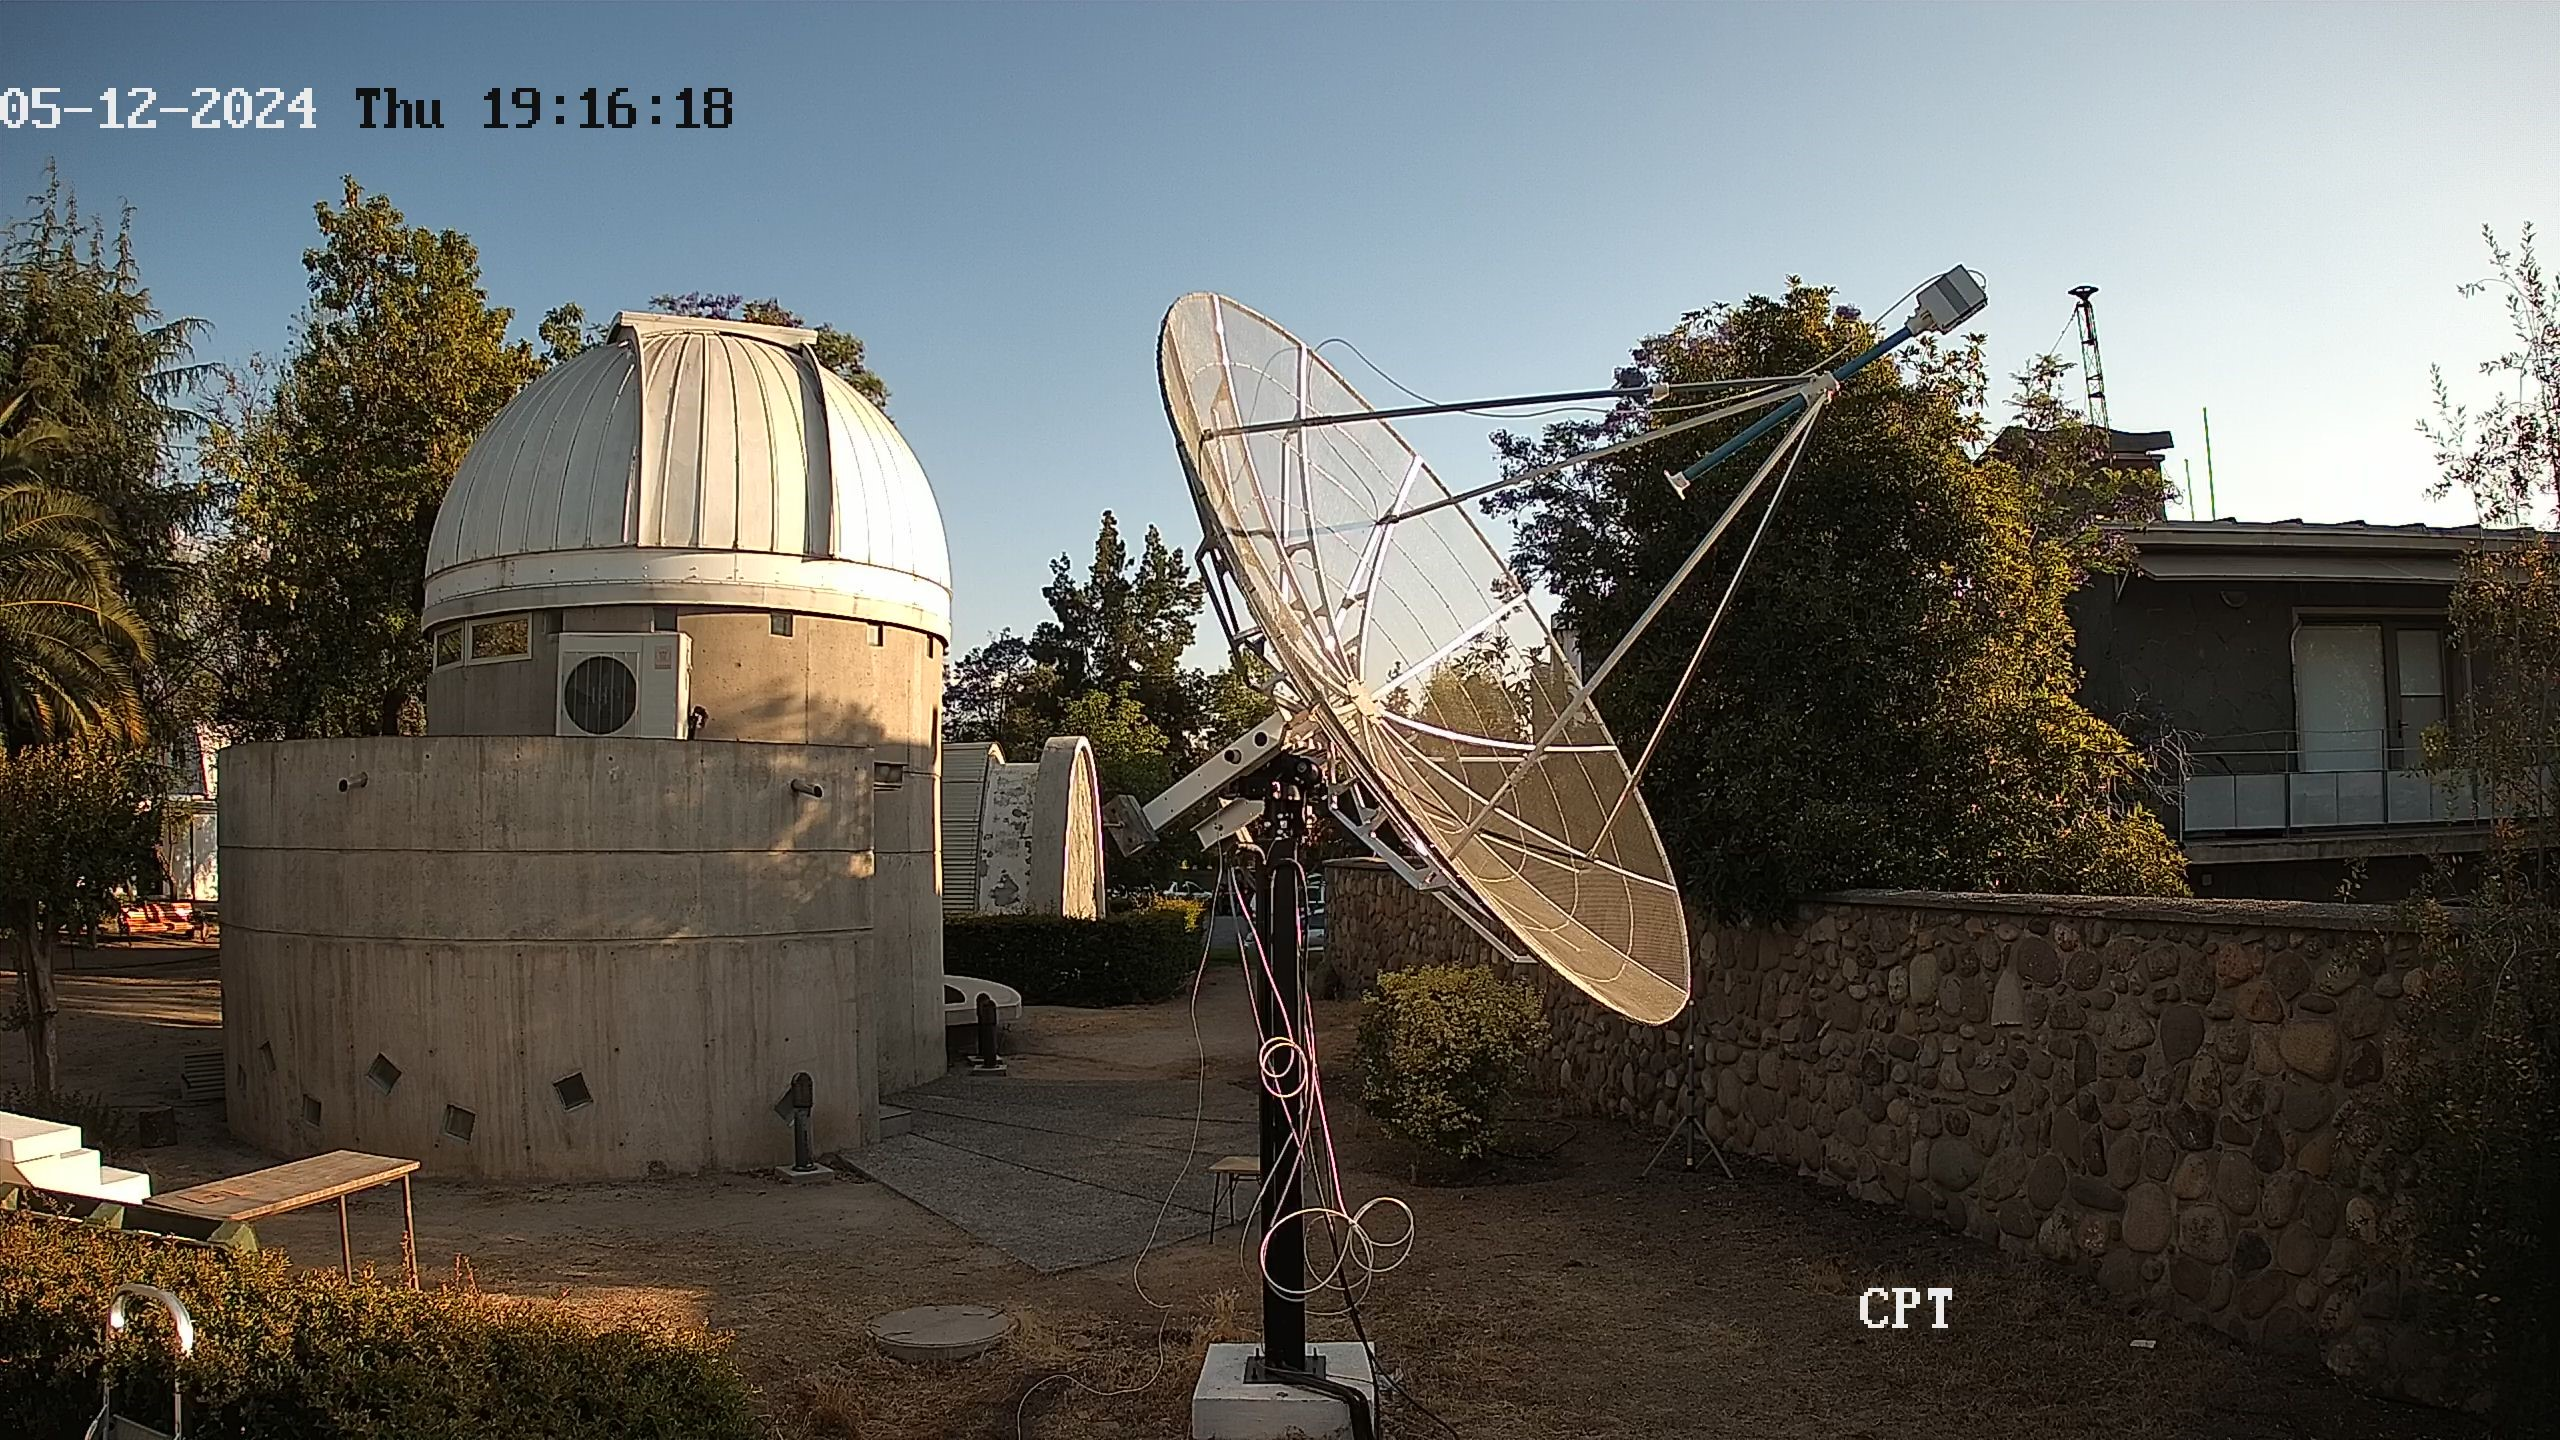
\includegraphics[width=0.8\textwidth]{img/antenna}
    \caption{Antena construida siendo monitoreada por la cámara remota}
    \label{fig:antena}
\end{figure}

\section{Posicion del alimentador}

La posición del alimentador con mayor ganancia se obtuvo a 135 cm de la superficie del reflector. La figura \ref{fig:distancia} muestra la ganancia en función de la distancia del alimentador al reflector.\\

\begin{figure}
    \centering
    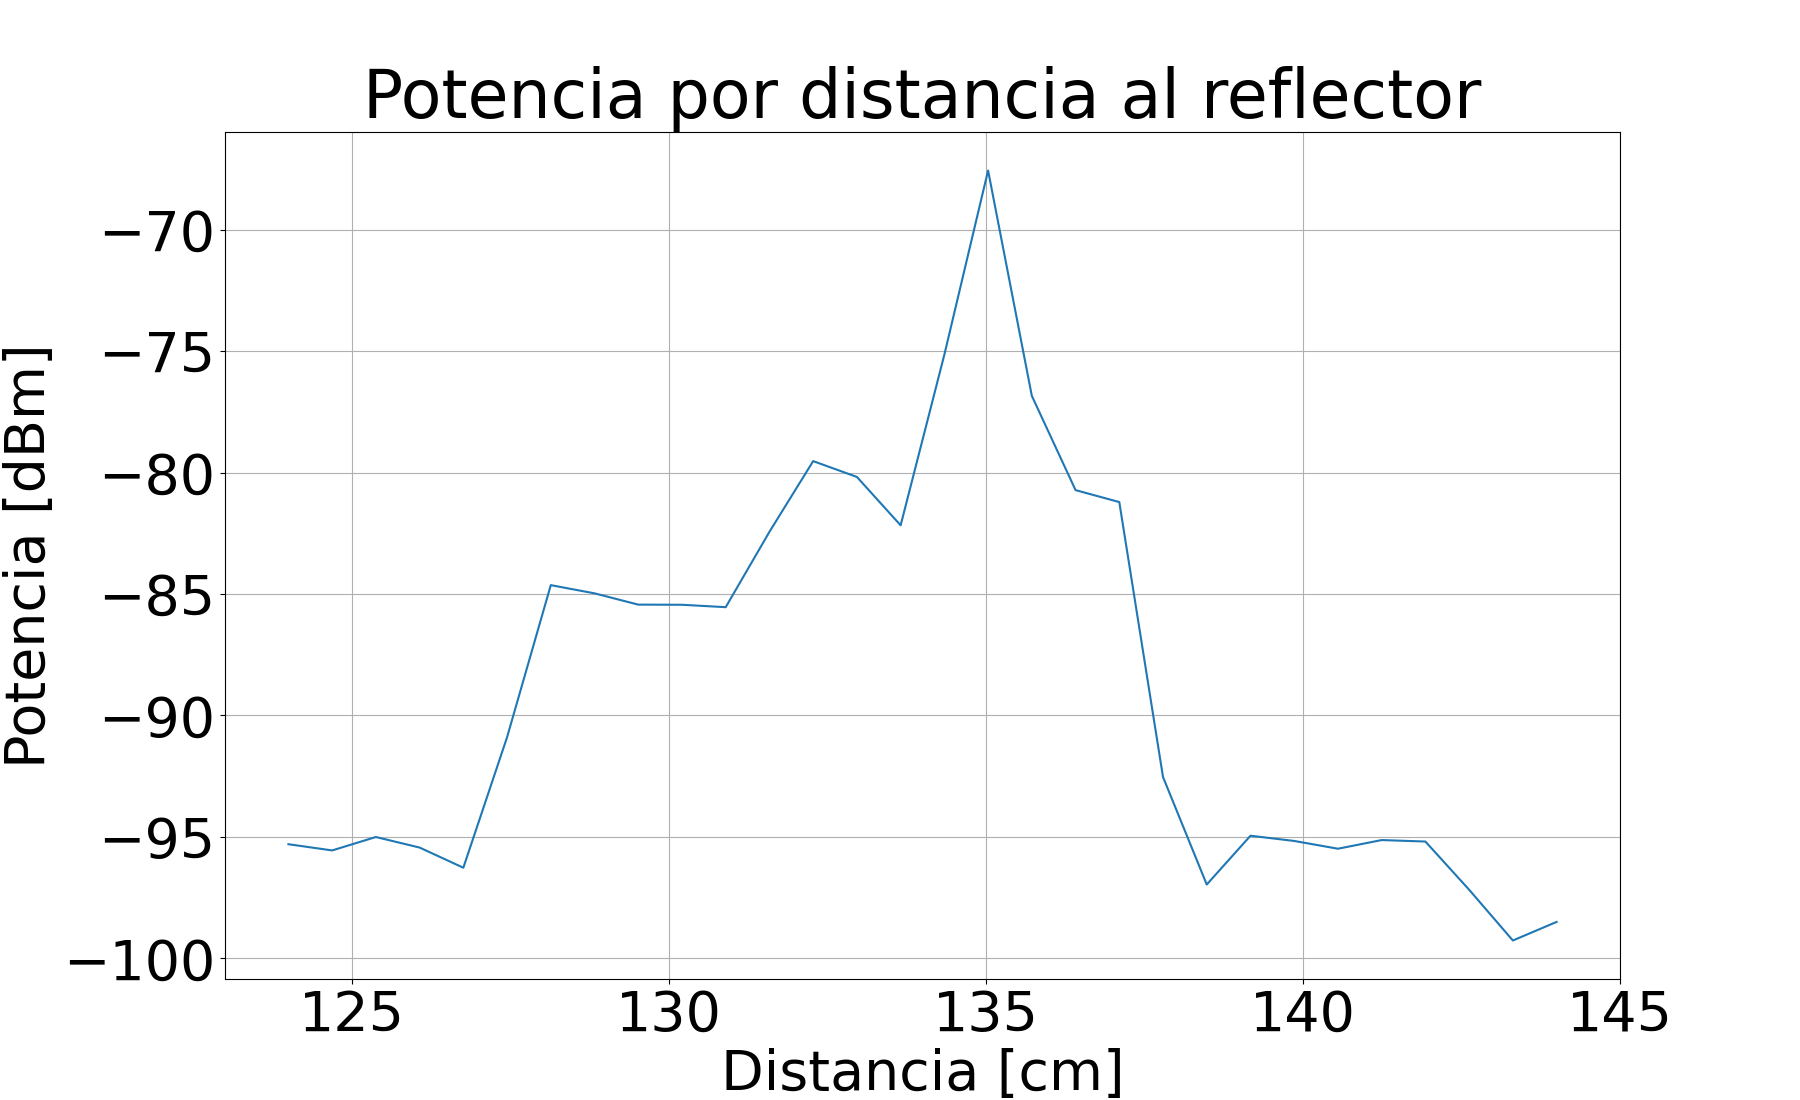
\includegraphics[width=0.8\textwidth]{img/enfoqueDist}
    \caption{Potencia recibida en función de la distancia del alimentador al reflector}
    \label{fig:distancia}
\end{figure}

La distancia obtenida coincide con la distancia focal de la antena y se observa que la a medida que el alimentador se aleja del foco, aumentando o disminuyendo la distancia con la parábola, la ganancia disminuye drásticamente perdiendo 6 dB por centímetro hasta llegar a la ganancia que tendría la antena sin considerar el reflector.\\

Estas pérdidas son análogas a la medida de 1420 MHz para la de 400 MHz.\\

\section{Patrón de radiación} \label{sec:patron}

A continuación, se presentan los patrones de radiación obtenidos para la antena a 1428 MHz y 400 MHz. Para la banda de 1428 MHz se realizaron los 2 cortes de elevación y azimuth ya que este se obtuvo utilizando el digitalizador del receptor, lo que permite hacer las maniobras de elevación completas. En cambio, para 400 MHz, se debía utilizar un cable coaxial hacia el analizador de espectro.\\

% \begin{figure}
%     \centering
%     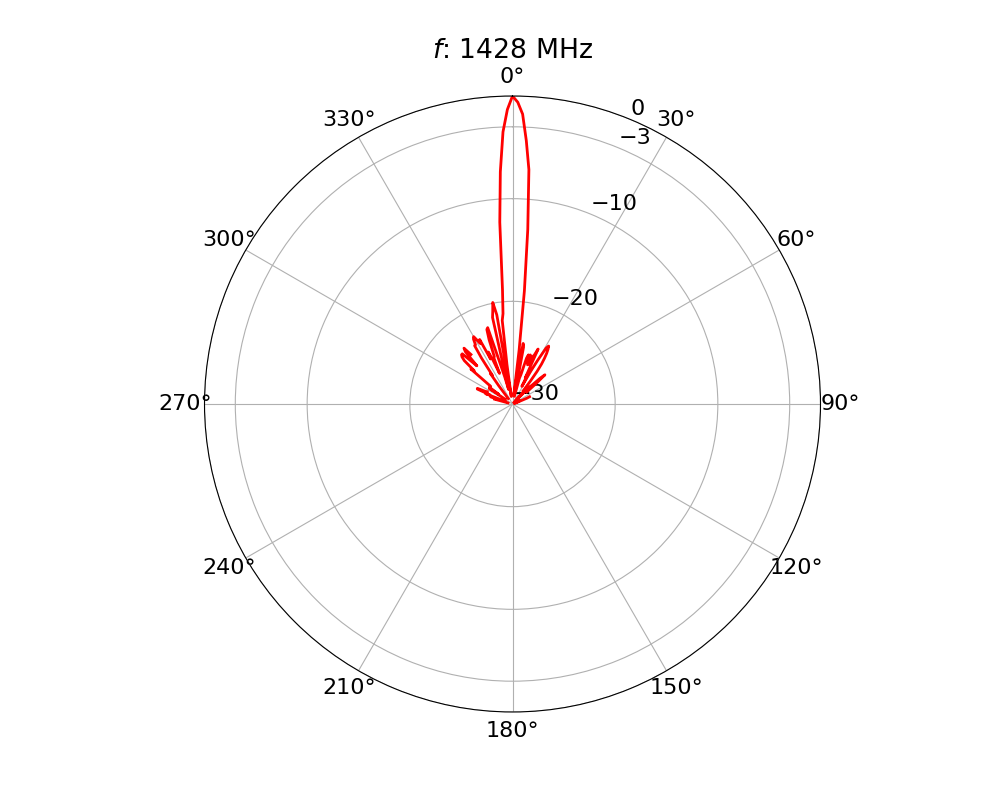
\includegraphics[width=0.8\textwidth]{img/1420rp}
%     \caption{Corte azimutal patrón de radiación a 1428 MHz}
%     \label{fig:1420rp}
% \end{figure}

% \begin{figure}
%     \centering
%     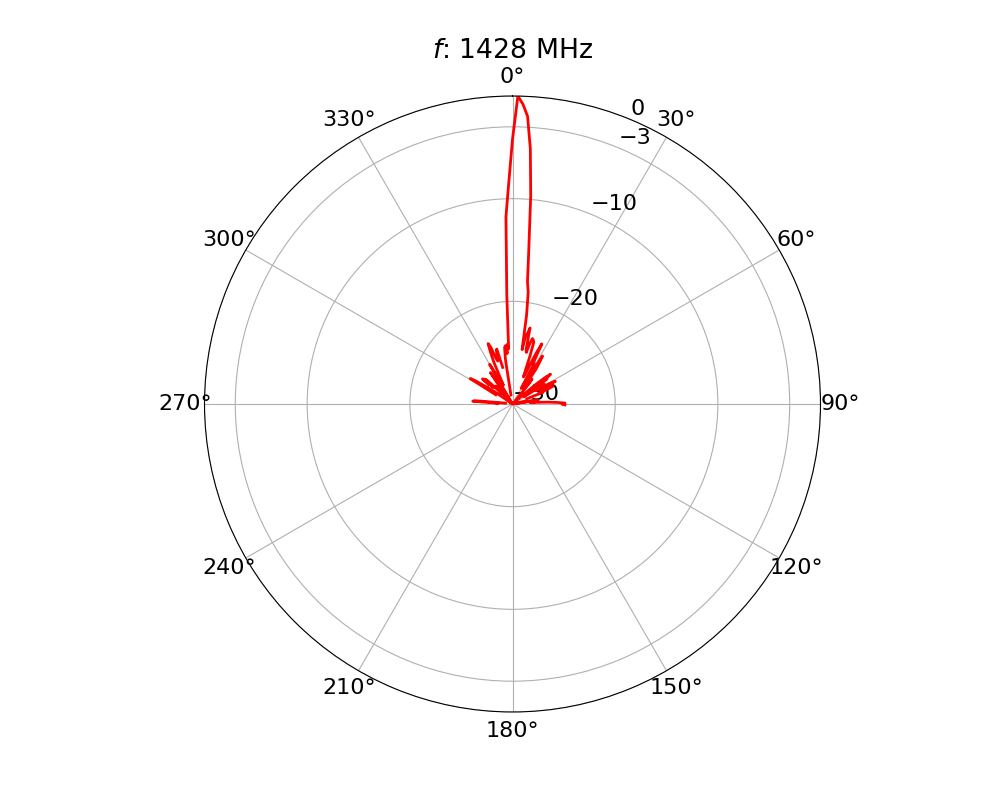
\includegraphics[width=0.8\textwidth]{img/1420rpel}
%     \caption{Corte elevacion patrón de radiación a 1428 MHz}
%     \label{fig:1420rpel}
% \end{figure}

\begin{figure}[h!]
    \centering
    \begin{subfigure}{0.45\textwidth}
        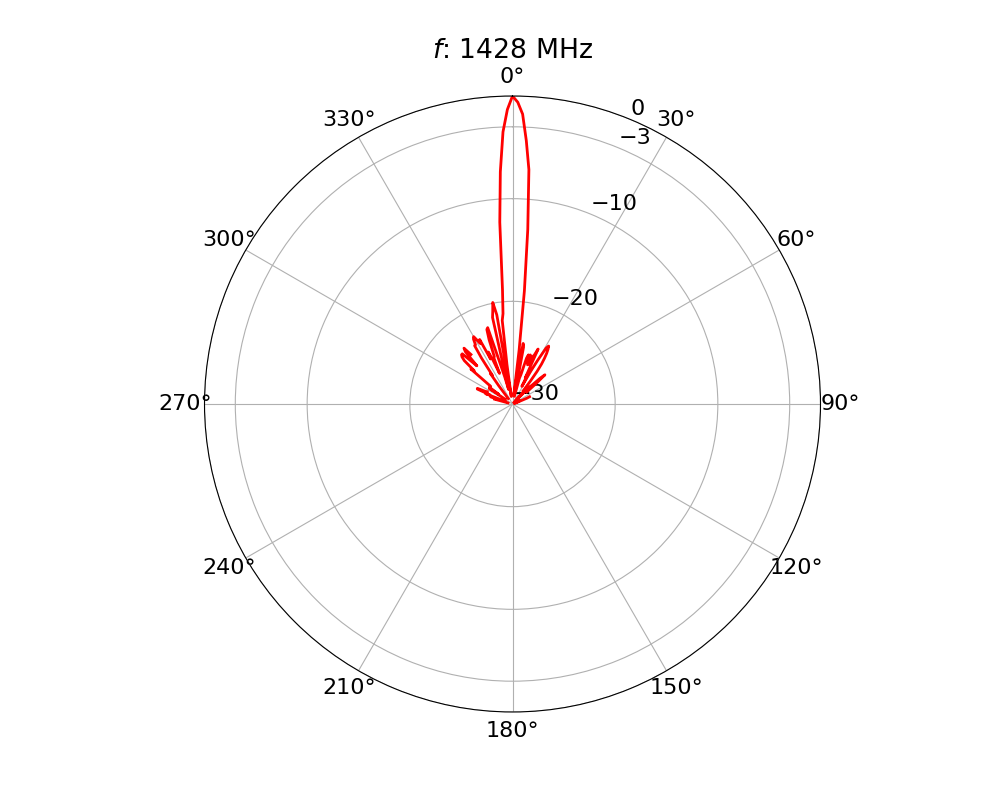
\includegraphics[width=\textwidth]{img/1420rp}
        \caption{Corte azimutal patrón de radiación a 1428 MHz}
        \label{fig:1420rp}
    \end{subfigure}
    \begin{subfigure}{0.45\textwidth}
        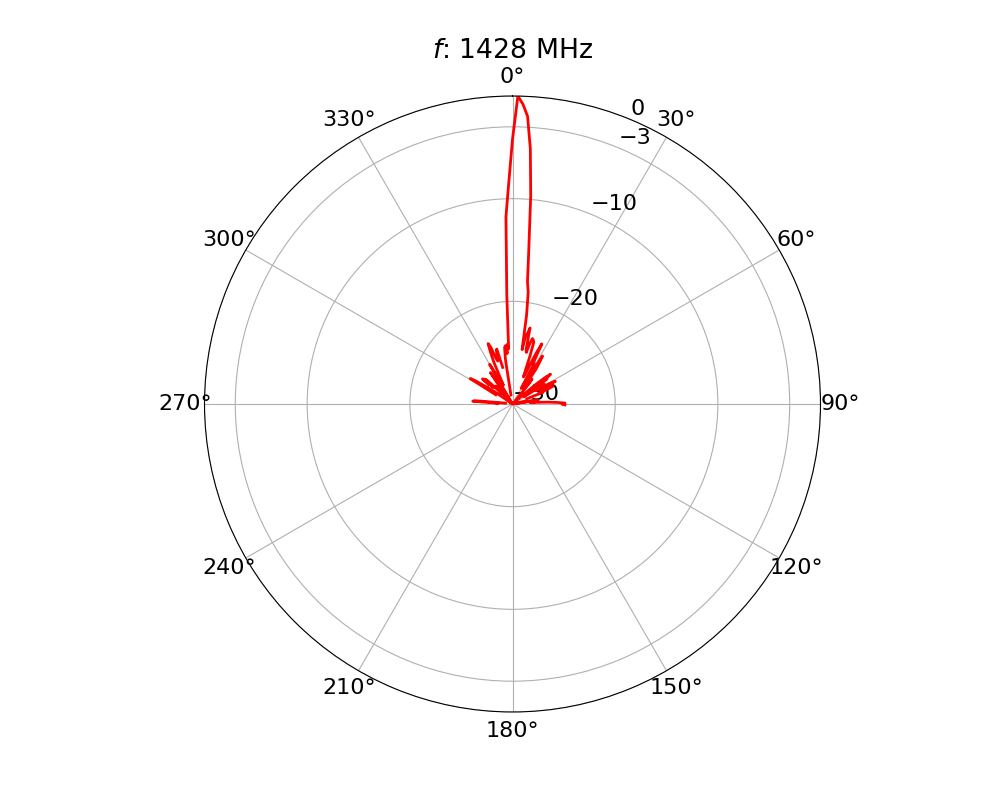
\includegraphics[width=\textwidth]{img/1420rpel}
        \caption{Corte elevacion patrón de radiación a 1428 MHz}
        \label{fig:1420rpel}
    \end{subfigure}
\end{figure}


%\begin{images}{Tono de -80 dBm a las frecuencias de interés}
%    \addimage{img/1420rp}{width=8cm}{}\label{fig:1420rp}
%    \addimage{img/1420rpel}{width=8cm}{}\label{fig:1420rpel}
%\end{images}



%\begin{figure}
%    \centering
%    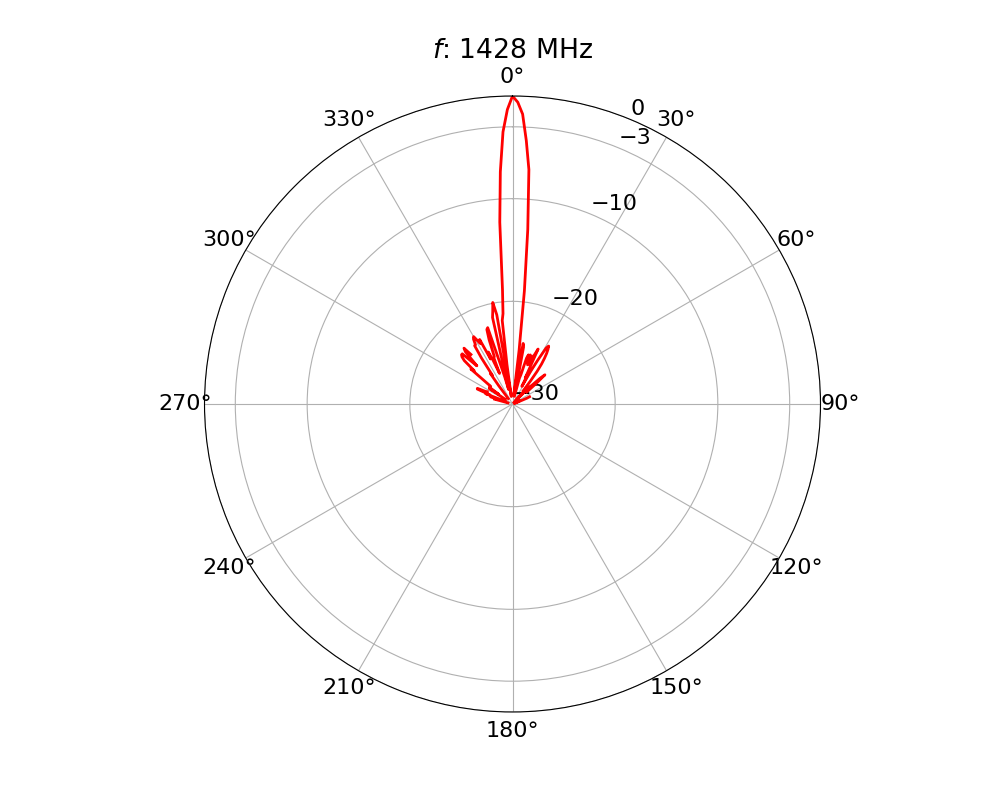
\includegraphics[width=0.8\textwidth]{img/1420rp}
%    \caption{Corte azimutal patrón de radiación a 1428 MHz}
%    \label{fig:1420rp}
%\end{figure}

En la figura \ref{fig:1420rp} se observa el corte azimutal del patrón de radiación a 1428 MHz, donde se aprecia un lóbulo principal predominante de 4.4 grados de HPBW y todos los demás lóbulos laterales bajo -20 dB.\\

%\begin{figure}
%    \centering
%    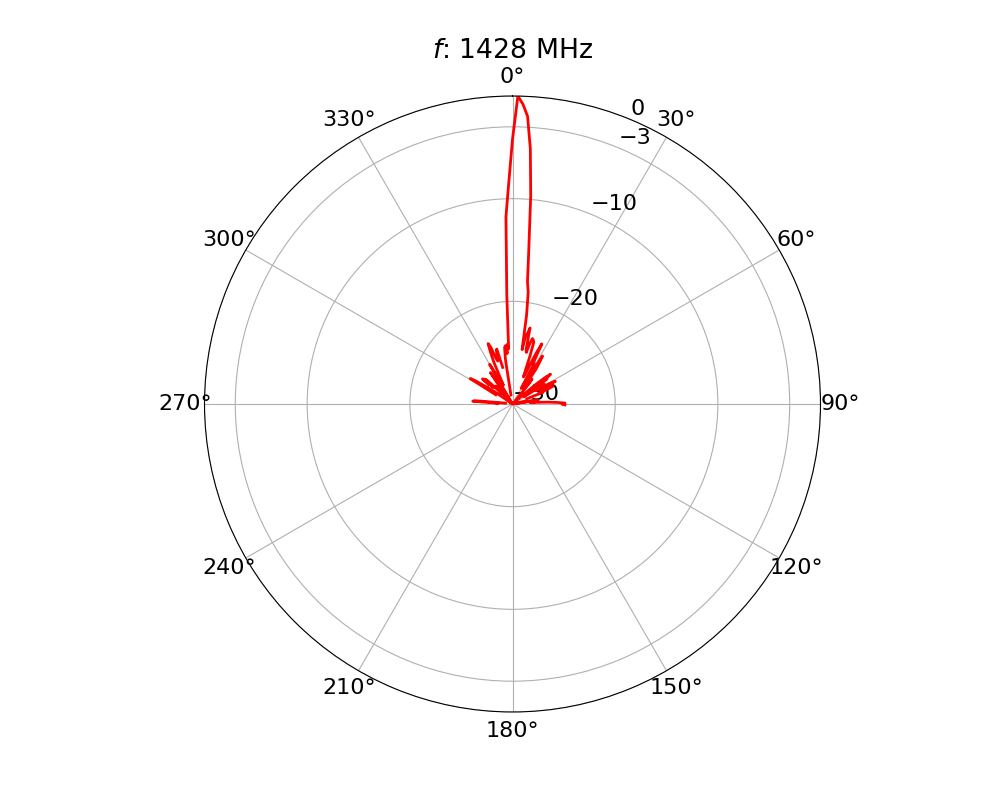
\includegraphics[width=0.8\textwidth]{img/1420rpel}
%    \caption{Corte elevacion patrón de radiación a 1428 MHz}
%    \label{fig:1420rpel}
%\end{figure}

Con respecto al corte de elevación, de la figura \ref{fig:1420rpel}, se observa un lóbulo principal de 4.3 grados de HPBW y una discontinuidad en el lóbulo principal a 0 grados. Los lobulos laterales  se encuentran por debajo de -25 dB.\\

%\begin{figure}
%    \centering
%    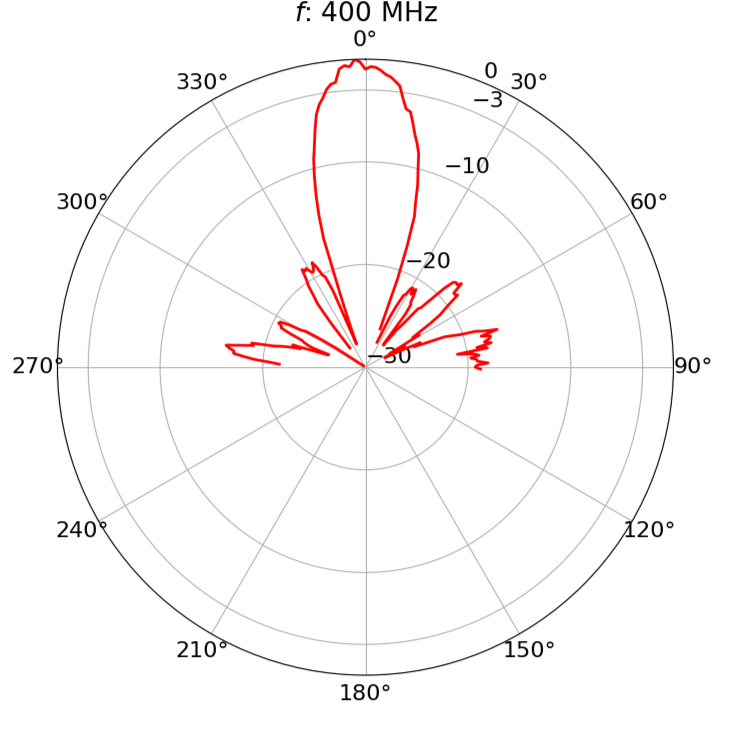
\includegraphics[width=0.8\textwidth]{img/400rp}
%    \caption{Corte azimutal patrón de radiación a 400 MHz}
%    \label{fig:400rp}
%\end{figure}

\begin{figure}[h!]
    \centering
    \begin{subfigure}{0.45\textwidth}
        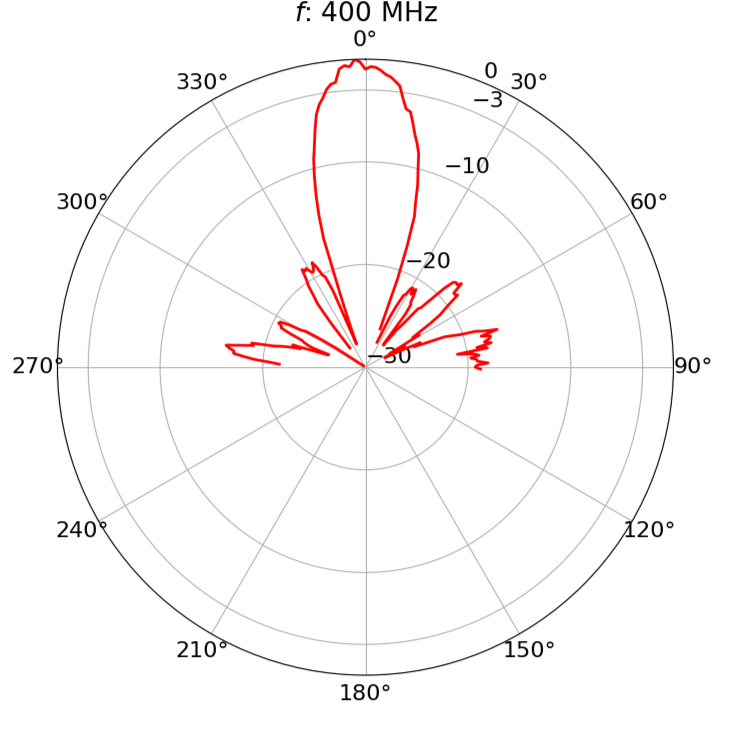
\includegraphics[width=\textwidth]{img/400rp}
        \caption{Corte azimutal patrón de radiación a 400 MHz}
        \label{fig:400rp}
    \end{subfigure}
    \begin{subfigure}{0.45\textwidth}
        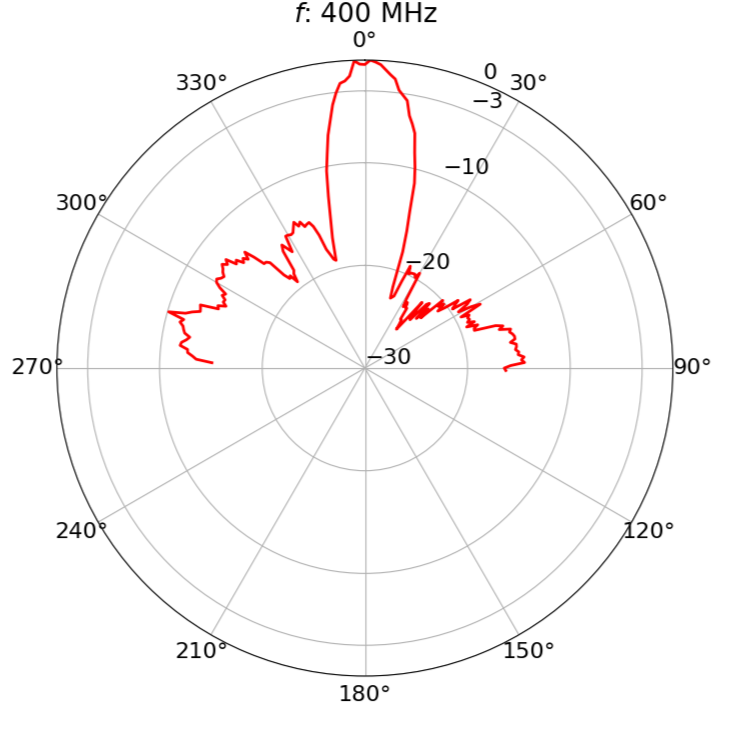
\includegraphics[width=\textwidth]{img/400rpel}
        \caption{Corte elevacion patrón de radiación a 400 MHz}
        \label{fig:400rpel}
    \end{subfigure}
\end{figure}


En la figura \ref{fig:400rp} se observa el corte azimutal del patrón de radiación a 400 MHz, donde se aprecia un lóbulo principal predominante de 7.5 grados de HPBW y todos los demás lóbulos laterales bajo -15 dB.\\

%\begin{figure}
%    \centering
%    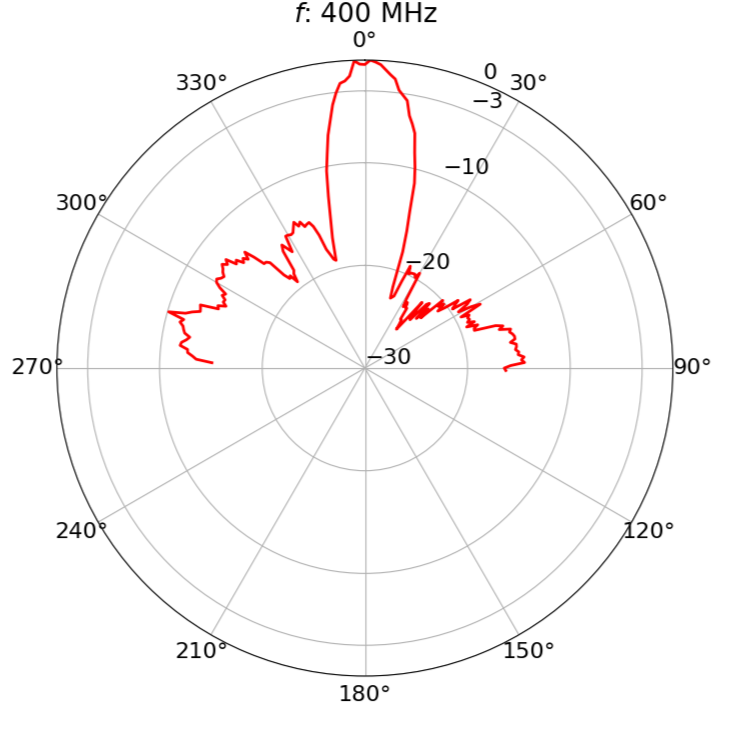
\includegraphics[width=0.8\textwidth]{img/400rpel}
%    \caption{Corte elevación patrón de radiación a 400 MHz}
%    \label{fig:400rpel}
%\end{figure}

Con respecto al corte de elevación, de la figura \ref{fig:400rpel}, se observa un lóbulo principal de 7.5 grados de HPBW y una discontinuidad en el lóbulo principal a 0 grados. A diferencia de la figura \ref{fig:400rp} los lóbulos laterales están dominados por ruido, sin embargo, sigue por debajo de los -15 dB\\



\section{Sensibilidad}

La radio definida por software, entrega una escala relativa de potencia o dBFS, por lo que se calibró la escala de potencia con la ayuda de un generador de señales.\\

\begin{figure}
    \centering
    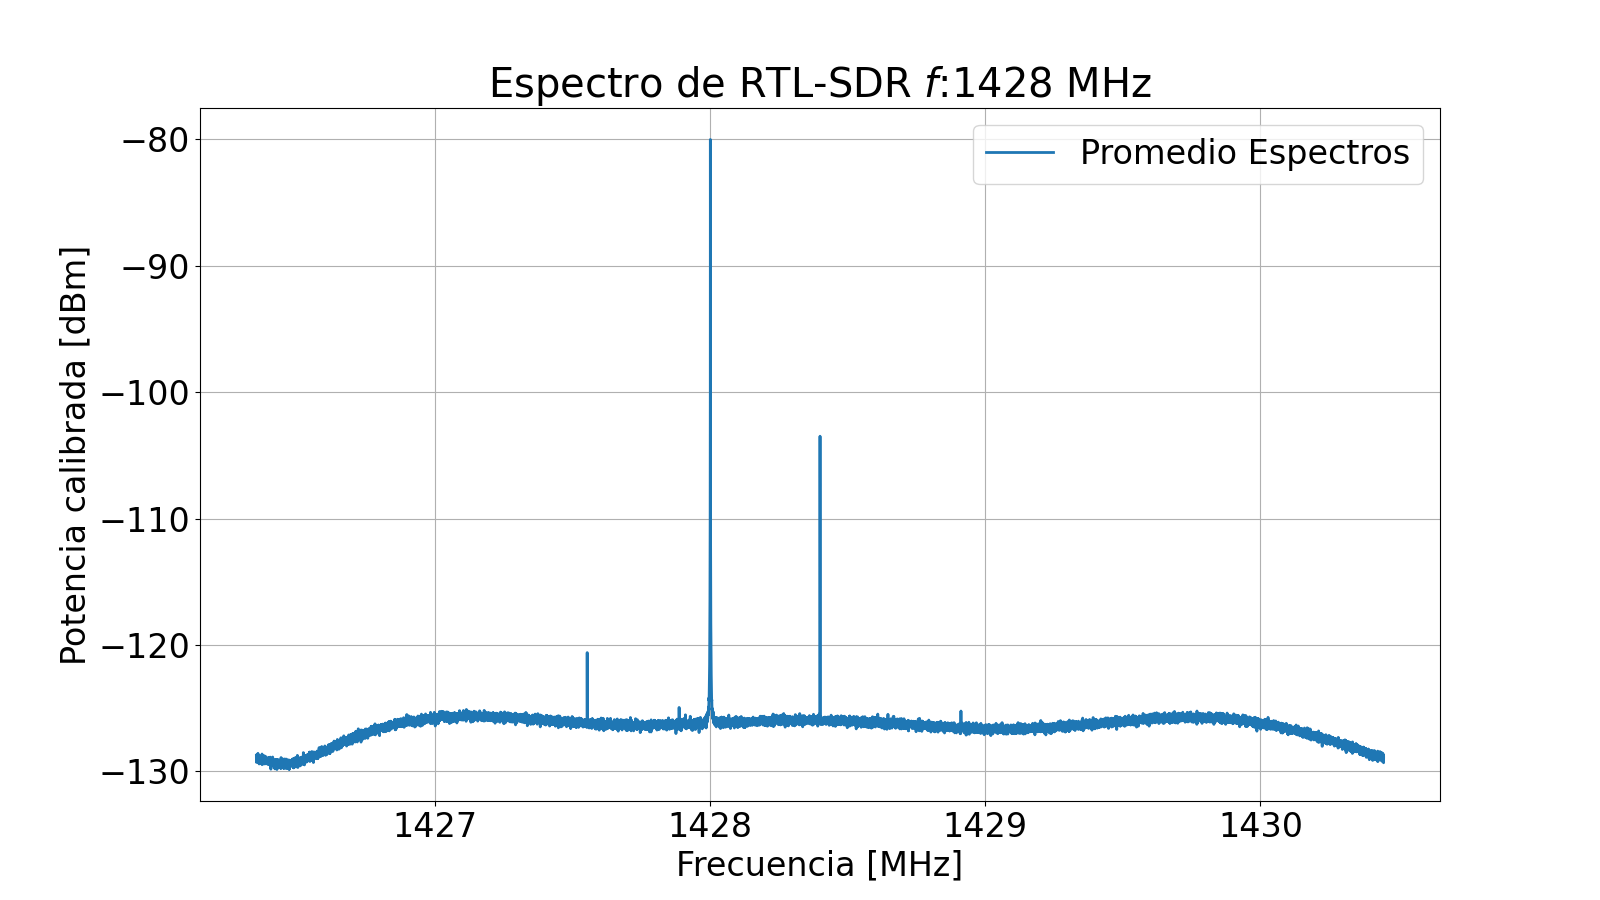
\includegraphics[width=0.8\textwidth]{img/rtl1428}
    \caption{Espectro obtenido por la RTL-SDR a 1428 GHz calibrado a potencia}
    \label{fig:rtl1428}
\end{figure}

Como se peude apreciar en la figura \ref{fig:rtl1428}, para la frecuencia específica de 1428 MHz, se calibró la escala para obtener los mismos -80 dBm que fueron inyectados, siendo la corrección obtenida de -40.7 dB.\\

Se repitio la medición de potencia en las demás frecuencias de interés, obteniendo los espectros de la figura \ref{rtl_specs} y las sigueientes correcciones de potencia para cada caso de la tabla \ref{tab:correccion}.\\

\begin{table}
    \centering
    \begin{tabular}{|c|c|c|}
        \hline
        Frecuencia (MHz) & Corrección (dB) & Pérdidas Ohmnicas (dB)\\
        \hline
        300 & -73.2 & 4.45\\
        400 & -70.63 & 5.2\\
        500 & -68.65 & 5.9\\
        1000 & -49.43 & 8.45\\
        1500 & -39.42 & 10.5\\
        1700 & -36.81 & 11.5\\
        \hline
    \end{tabular}
    \caption{Corrección de potencia para las frecuencias de interés}
    \label{tab:correccion}
\end{table}


\begin{images}{Tono de -80 dBm a las frecuencias de interés}
    
    \addimageanum{img/rtl300}{width=8cm}
    \addimageanum{img/rtl1000}{width=8cm}

    \imagesnewline

    \addimageanum{img/rtl400}{width=8cm}
    \addimageanum{img/rtl1500}{width=8cm}

    \imagesnewline

    \addimageanum{img/rtl500}{width=8cm}
    \addimageanum{img/rtl1700}{width=8cm}

    \label{fig:rtl_specs}
\end{images}

\section{Ganancia y Directividad}

Al considerar una apertura de 3 metros de diámetro, se calculó la directividad a partir de definición teórica para la banda de 1428 MHz.\\

\begin{equation}
    D = \frac{4\pi A}{\lambda^2} = 2033.7
\end{equation}

También se calculó la directividad a partir de los haces de media potencia obtenidos en la sección \ref{sec:patron}, utilizando la aproximación de apertura circular uniforme para un reflector parabólico.\\

\begin{equation}
    D = \frac{38,933}{HPBW_{E}\cdot HPBW_{H}} = 2057.7
\end{equation}

Lo que se condice con el valor teórico con un error aproximado de un 1\%.\\

Luego utilizando las mediciones de potencia en la banda de 1428 MHz, una vez calibradas con la escala obtenida con la RTL-SDR en la figura \ref{fig:rtl1428}, se obtuvo una ganancia del sistema a partir de la ecuación de Friis con la estrella artificial.\\

La potencia inyectada en la antena de 3 dBi de la copa de agua fue de 2.23 dBm, el cable de 20 metros de longitud y el cable de 2 metros tiene una atenuación de 20.4 dB y 2.2 dB respectivamente a la frecuencia de 1428 MHz, las pérdidas de espacio libre son de 81.01 dB y la potencia medida en el receptor fue -67.22 dBm.\\

\begin{equation}
    P_{rx}(dBm) = P_{tx}(dBm) + G_{tx}(dB) + G_{rx}(dB) - 20log{R}(km) - 20log{f}(MHz) - L_{\Omega}(dB)
\end{equation}

\begin{equation}
    G_{rx} = -67.22 -2.23 - 3 + 81.01 + 20.4 + 2.2 = 31.16 (dB)
\end{equation}

Con lo que se obtiene una ganancia de 31.16 dB para la banda de 1428 MHz. Por consecuencia se puede determinar la eficiencia de apertura considerando la directividad obtenida a partir del patrón de radiación de $D=2057.7$.\\

\begin{equation}
    \varepsilon_{A} = \frac{G}{D} = \frac{1304.1}{2057.7} = 0.634
\end{equation}

\begin{equation}
    \varepsilon_{A} = 0.634
\end{equation}

Este valor de eficiencia de apertura en comparación con la eficiencia de apertura declarada por el fabricante es un poco menor, siendo la del fabricante de 0.65 para el rango de frecuencias entre 1.2 a 4 GHz.\\

\section{Error de apuntamiento}

El máximo de potencia recibida se obtuvo al comandar una posición de 7 grados de elevación con 171 grados de azimuth. La posición determinada de la fuente con respecto a la ubicación del telescopio es 4.6 grados de elevación y 6 grados de azimuth.\\

La diferencia entre la posición de la fuente y la posición de la antena es de 2.4 grados en elevación y 3 grados en azimuth. Así el error de apuntamiento es de +2.4 grados y +3 grados de elevación y azimuth respectivamente.\\

%\section{Ancho de banda}

\section{Primera luz}

\begin{figure}
    \centering
    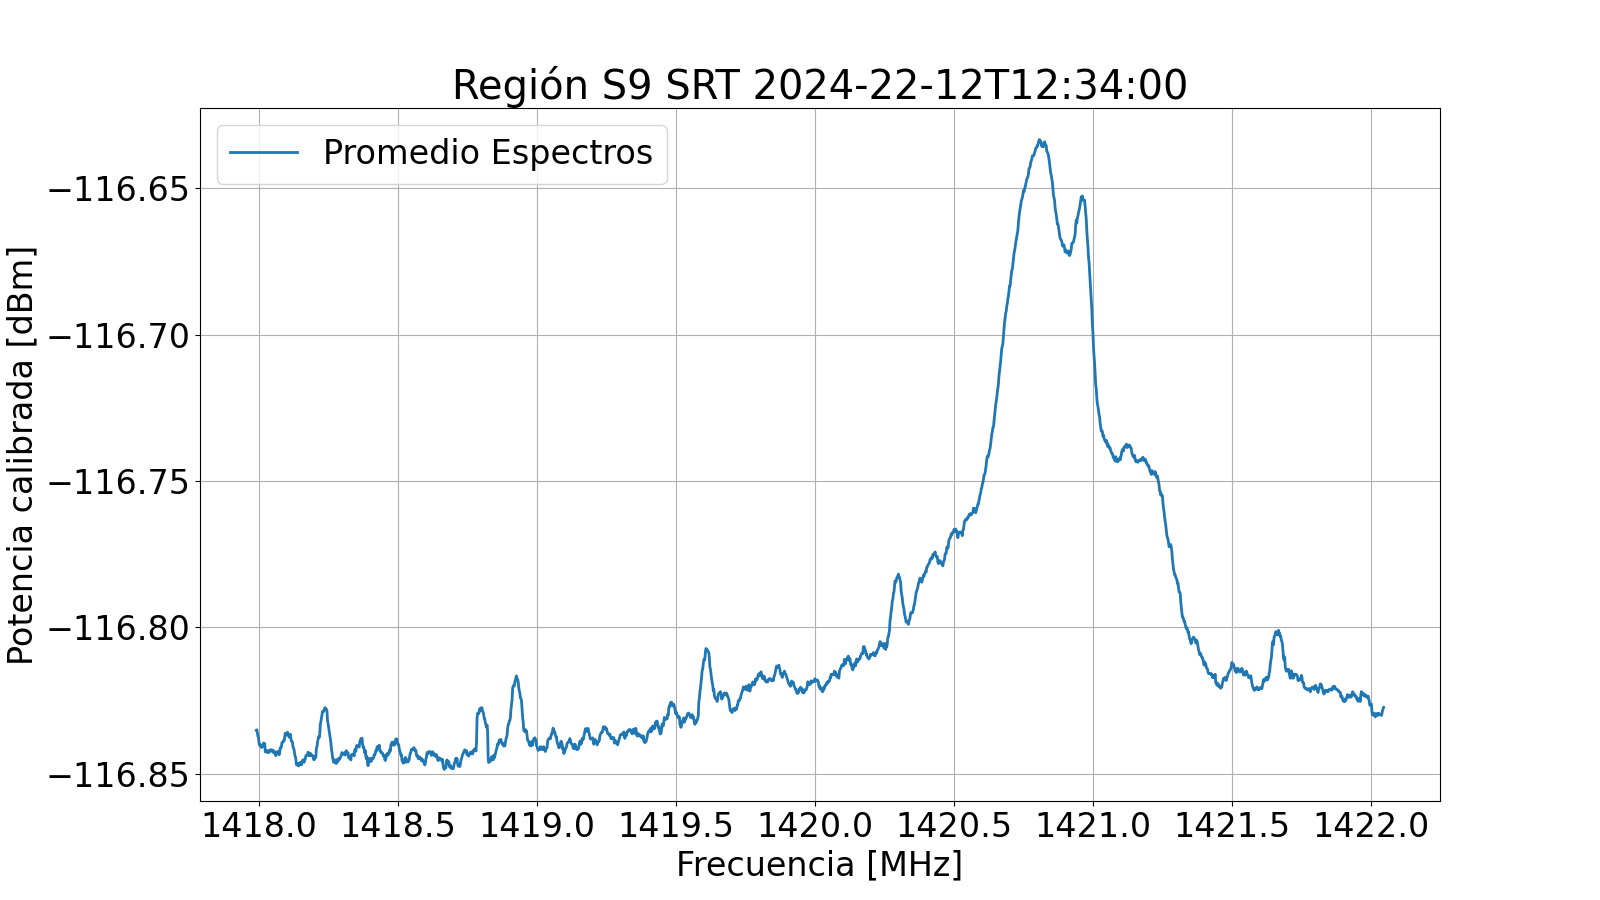
\includegraphics[width=0.8\textwidth]{img/h1}
    \caption{Espectro obtenido por la RTL-SDR a 1420 MHz calibrado a potencia}
    \label{fig:firstlight}
\end{figure}

En el spectro de la figura \ref{fig:firstlight} se observa la curva de H1 obtenida en la región estandar S9. Se aprecia un máximo de potencia recibida con 0.2 dB sobre el piso de ruido del receptor centrado en 1420.7 MHz. También se pueden distinguir picos de interferencia de radiofrecuencia en 1418.3 MHz, 1419 MHz, 1419.6 MHz y 1421.6 MHz.\\